This chapter provides detailed specifications of the system under development.

\section{Functional Requirements}
This section describes each function/feature provided by our system. These functions are logically grouped into modules based on their purpose/users/mode of operations etc (as per our system). A functional hierarchy may look like:
\begin{outline}
  \1 Login/Signup Module
  \2 The user should be able to login to the system
    \3 The software should automatically and immediately validate user credentials against the database system
    \3 After verification, the software should grant access to the user’s account only if all the credentials of the user match. 
  \2 The user should be able to create a new account (Signup)
    \3 The software should write the credentials for this new account in the database.
    \3 After storing the credentials, the software should grant access to this new account. 
  \2 The user should be able to change their password.
    \3 The software should update the password entry for the corresponding username in the database. 

 \1 Interface requirements
  \2 If the user has access to the account, they should be able to see the home screen of the software. The home screen will mainly give user the option to select between two options \textit{Training} and \textit{Fighting}.
  \2 The training session contains numbered lessons. Each lesson contains tutorials and practice sessions. 
  \2 The fighting session also contains numbered fights. Each fight $x$ requires the user to know the techniques included in lesson 1 till lesson $x$. A fight session is like a game in which user fights with the avatar. The avatar and the user, both have their health bars, which decreases if any of them fails to defend themselves against an opponent's attack. The fight session ends if either the user or avatar’s health bar gets empty. 
  \2 The user should be able to view the unlocked lessons. Lesson 1 will be unlocked by default and completing a lesson will unlock the next one. 
  \2 The user should be able to start the fight sessions of the corresponding unlocked lessons. 
  \2 The user should be able to view all the tutorials of an unlocked lesson. These tutorials are animated videos that teach the user a specific technique of self-defense. 
  \2 The user should be able to practice any of the tutorials from the unlocked lessons. This practice session is only of a specific technique which the tutorial teaches. 
  \2 If the user selects the haptic option for practice and fight session, they should be able to feel the interaction with the avatar after properly calibrating all the signal parameters.
  \2 The user should be able to see the feedback generated after a practice session ends. The feedback should be both visual and textual.
  \2 The user should be able to start a fight session of an unlocked lesson.
  \2 The user should be able to see the feedback generated after a fight session ends; the feedback should be visual and textual both.
  \2 The user should be able to see suggested tutorials to practice after fight session. These tutorials are the areas in which user needs improvement. 
  
 \1 Practice Session
   \2 If the user chooses to practice a specific tutorial, the avatar will attack, requiring the user to perform that specific technique which the tutorial teaches.  After the avatar is done performing the attack, the practice session will end giving detailed feedback to the user of his performance. 
 
 \1 Pose Detection Module
   \2 If the user selects to practice a tutorial or fight with avatar, the system should be able to extract stick figure data of their movement via OpenPose and a webcam/camera.
     \3 The system should first convert the live video to a series of images to be processed at a certain frequency. 
     \3 The system should then use OpenPose to generate stick figure for those images.
 \1 Feature Extraction Module
 `\2 Based on generated stick figures, extract useful features like rotation, velocity to be used for further analysis.
 \1 Pose Classification Module
  \2 Since the user is just practicing a single known move in practice session, the system does not need to classify the performed pose for practice session. For fight session, however, in order for pose evaluation to take place, we first need to classify the pose into one of the stored poses.
  \2 In fight session, since the user will be performing several moves at the same time in response to avatar’s attacks, each performed move by the user will be classified. After classification of each performed move, each will go through pose evaluation module to get feedback feedback on his moves separately rather than one combined feedback. 
  
 \1 Pose Evaluation Module
  \2 The system should be able to evaluate the different moves performed by the user in practice and fight sessions.
    \3 The system should use the extracted features to calculate a score indicating how well the user performed a particular move by comparing it against the benchmark.

 \1 User Feedback Module
  \2 The user should be able to get visual feedback
    \3 The visual feedback consists of difference between the performed pose (stick figure) at an instant (the time instant where user made a mistake) and the stored pose (stick figure). The stored (correct) pose will be displayed in green and the part of the user’s pose will be displayed in red which do not properly align with the stored ones.  
  \2 The user should be able to get textual feedback 
   \3 The textual feedback will consist of a natural language feedback, which will tell the user what he/she lacked and how they can improve. 

 \1 Adaptive Teaching Module
  \2 The tutorials suggested by the system for more practice should be based on the low pose evaluation scores. 

 \1 Haptic Feedback Module
  \2 The system should be integrated with the haptic hardware.
  \2 The user should be able to calibrate the signal parameters for haptics that best comforts them.
  \2 The user should not penetrate into the avatar’s body.
  \2 The user should feel the impulse feedback on his arms and fists. 
\end{outline}

% --- The above is to be modified as per your project, e.g. a flat list if your system has limited functional requirements.

\section{Non-functional Requirements}
Following are the non-functional requirements of our system.
\subsubsection{Compatibility}
Software should be able to work on any laptop or computer with a camera.
\subsubsection{Usability}
The software should be user friendly and easy to navigate; no prior knowledge in the domain of Computer Science or self defense should be required for the user to experience the environment. 
\subsubsection{Modifiability}
The software can be expanded to other skills and functionalities, for instance additional defense techniques, if needed.
\subsubsection{Credibility}
Users can change their login password anytime they want; the new credentials must be updated in the database. 
\subsubsection{Integrability}
All components, whether they be software or hardware, should be integrated efficiently to ensure the smooth flow of the program when it is run. 
\subsubsection{Independability}
Besides being able to work as a complete, integrated project, the different components within the hardware should be able to function independently as well. For example, if one component of hardware fails, the other components should keep working. 
\subsubsection{Performance}
The program should provide a quick response time. It will be receiving user performance data in real-time and should respond to the user with relevant feedback in a matter of seconds.  
\section{External Interfaces}

\subsection{User Interfaces}
This section includes our mockup screens and briefly explains them. Figure \ref{fig:startingScreens} shows our screens for login/signup functionality. The software launches with a logo screen shown in figure \ref{fig:logo} which slowly fades out to display the login screen in figure \ref{fig:login}. If the user doesn't remember their password, they can change it through the change password screen in figure \ref{fig:password}. If the user does not have an account already, they can make a new account through the signup screen shown in figure \ref{fig:singup}.
    \begin{figure}[ht] 
  \subfigure[Logo Screen]{% 
    
\includegraphics[scale=0.25]{images/Mockups/logo.png} \label{fig:logo} 
  } 
 \quad 
  \subfigure[Signup Screen]{% 
    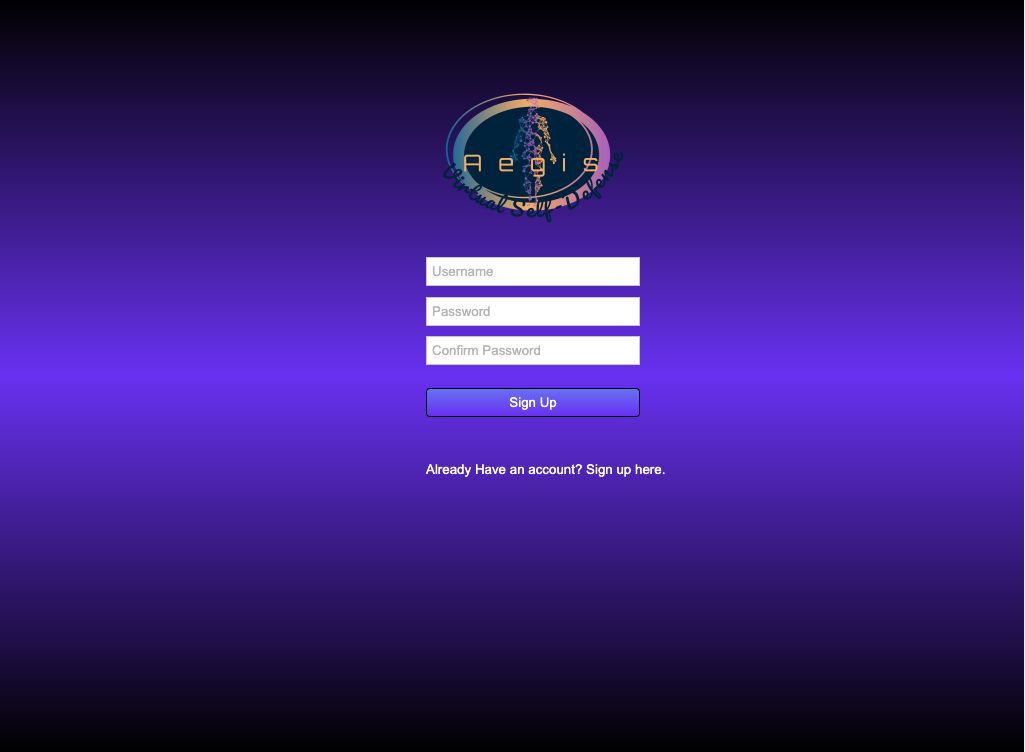
\includegraphics[scale=0.25]{images/Mockups/signup.png} \label{fig:singup} 
  } 
  \quad 
  \subfigure[Login Screen]{% 
    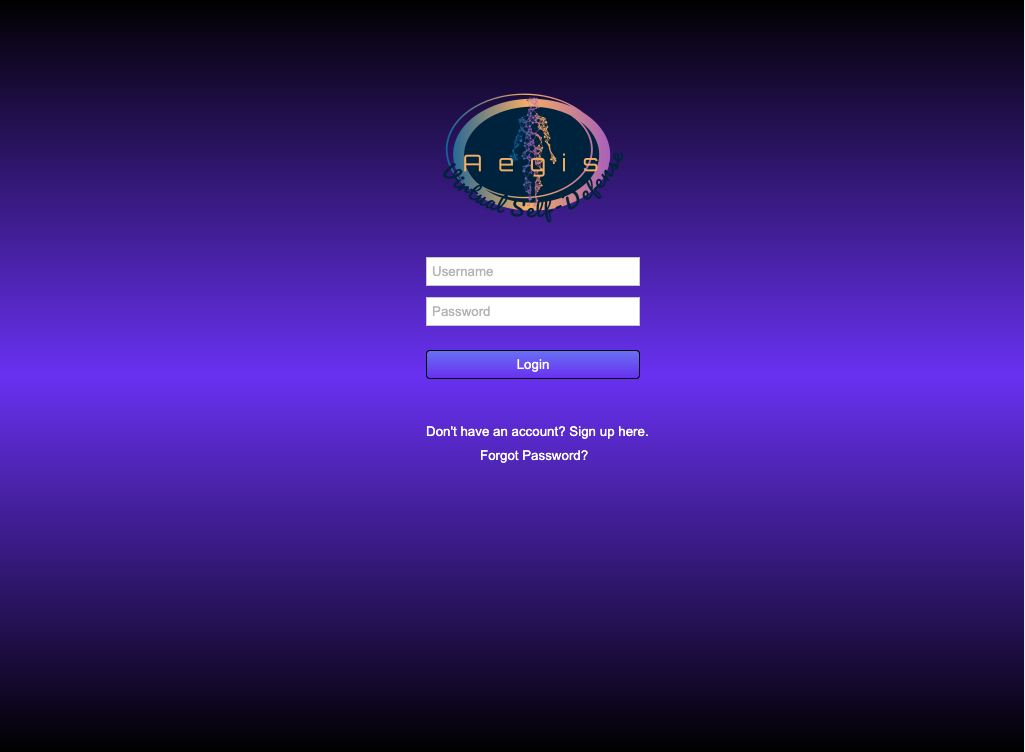
\includegraphics[scale=0.25]{images/Mockups/login.png} \label{fig:login} 
  }
  \quad 
  \subfigure[Change Password Screen]{% 
    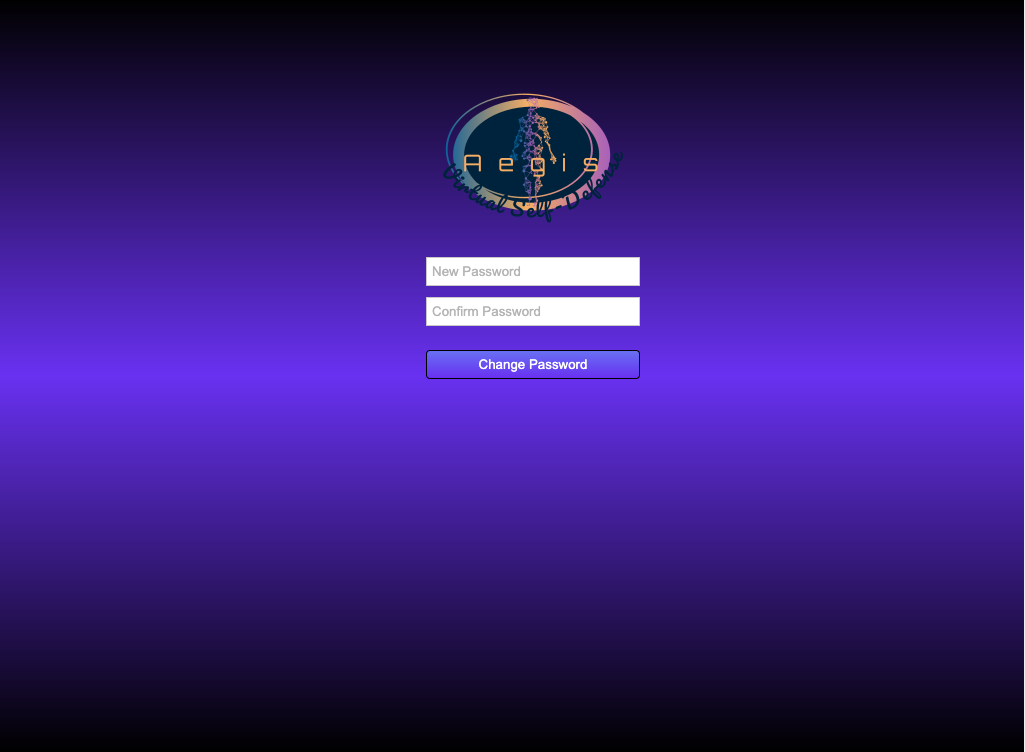
\includegraphics[scale=0.25]{images/Mockups/password.png} \label{fig:password} 
  }
  \caption{Login/Signup Functionality} 
  \centering
  \label{fig:startingScreens}
\end{figure}
\clearpage
Figure \ref{fig:homeTut} shows multiple screens related to home and \textit{Lesson 1} videos. After the user has been granted access to their account, home screen as shown in figure \ref{fig:home} is displayed. This screen gives user the option to choose between \textit{Training} or \textit{Fight} mode. Figure \ref{fig:lesson} shows the screen from where the user can navigate to introductory session of \textit{Lesson 1}, its tutorials and fight session. Screen in figure \ref{fig:intro} will guide the user what they will be learning in \textit{Lesson 1} which will be an animated video. Screen in figure \ref{fig:tutorial} will also display an animated video to the user guiding how a certain technique (specific to that tutorial) should be performed. 
    \begin{figure}[ht] 
  \subfigure[Home Screen]{% 
    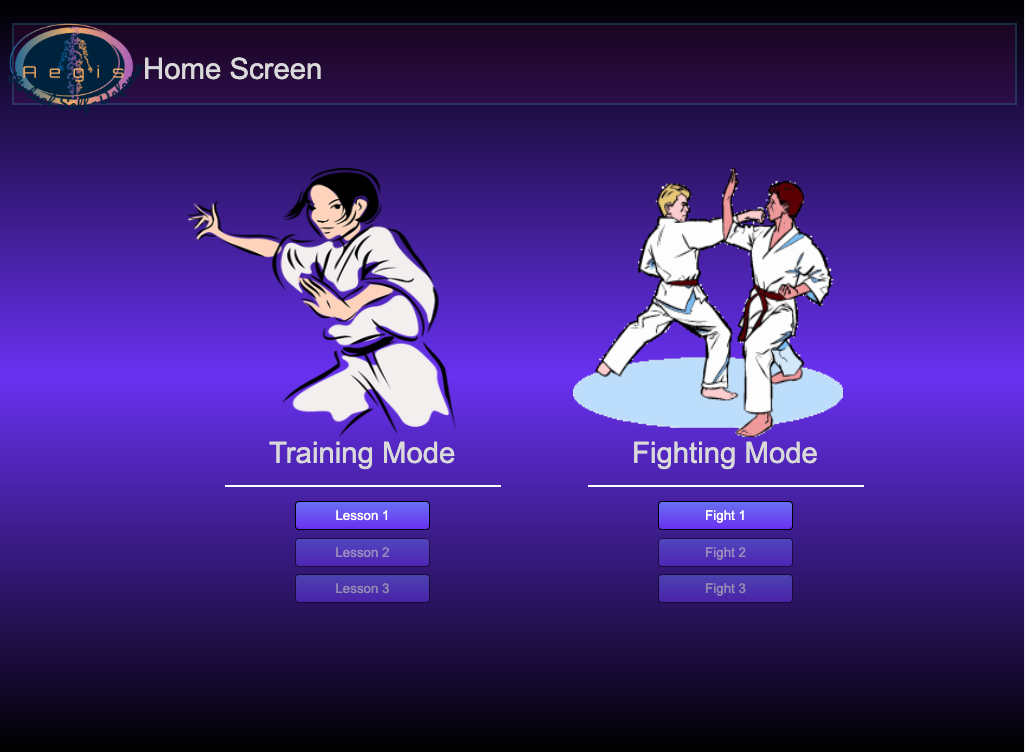
\includegraphics[scale=0.25]{images/Mockups/home.png} \label{fig:home} 
  } 
 \quad 
  \subfigure[Lesson I Screen]{% 
    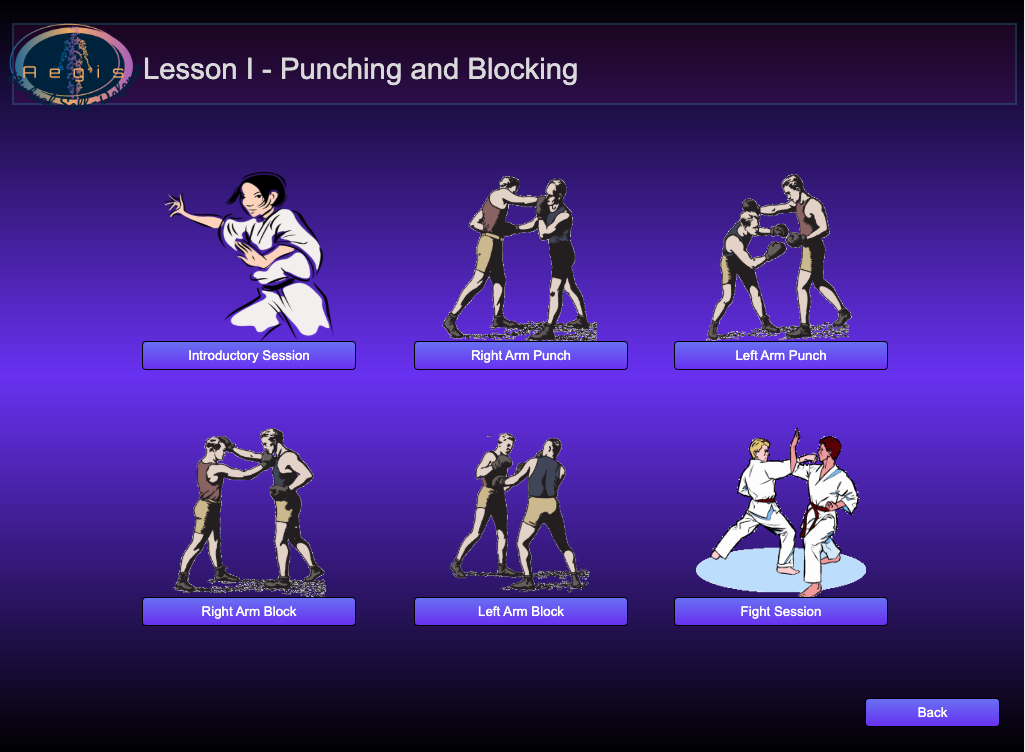
\includegraphics[scale=0.25]{images/Mockups/lesson.png} \label{fig:lesson} 
  } 
  \quad 
  \subfigure[Lesson I: Intro Screen]{% 
    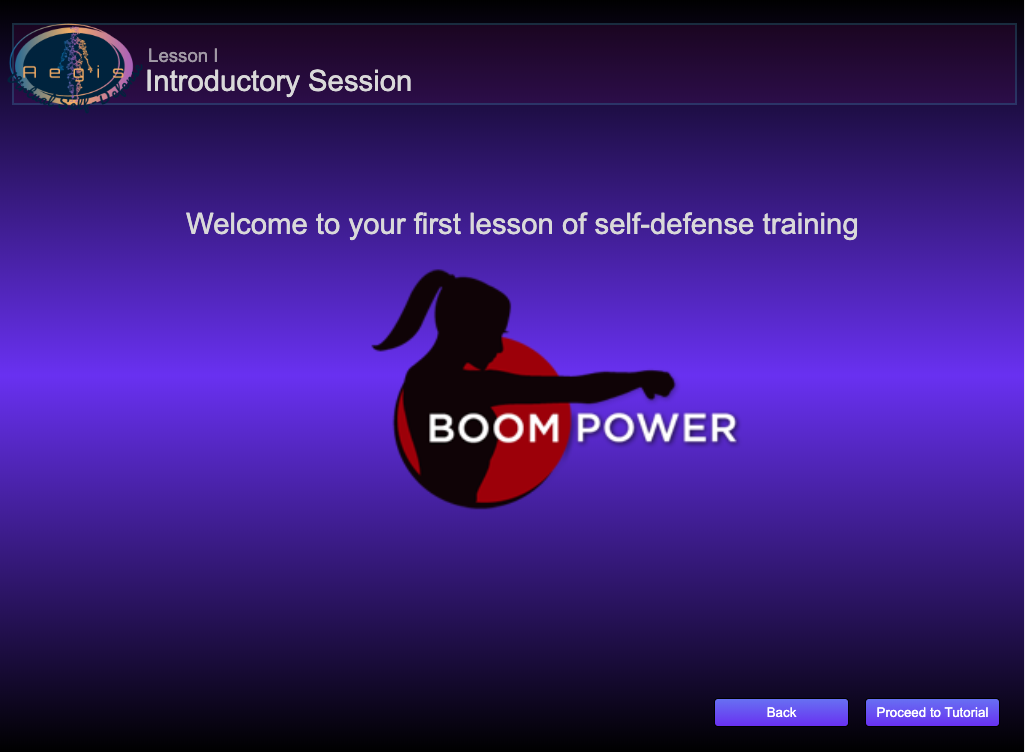
\includegraphics[scale=0.25]{images/Mockups/intro.png} \label{fig:intro} 
  }
  \quad 
  \subfigure[Lesson I: Tutorial I Screen]{% 
    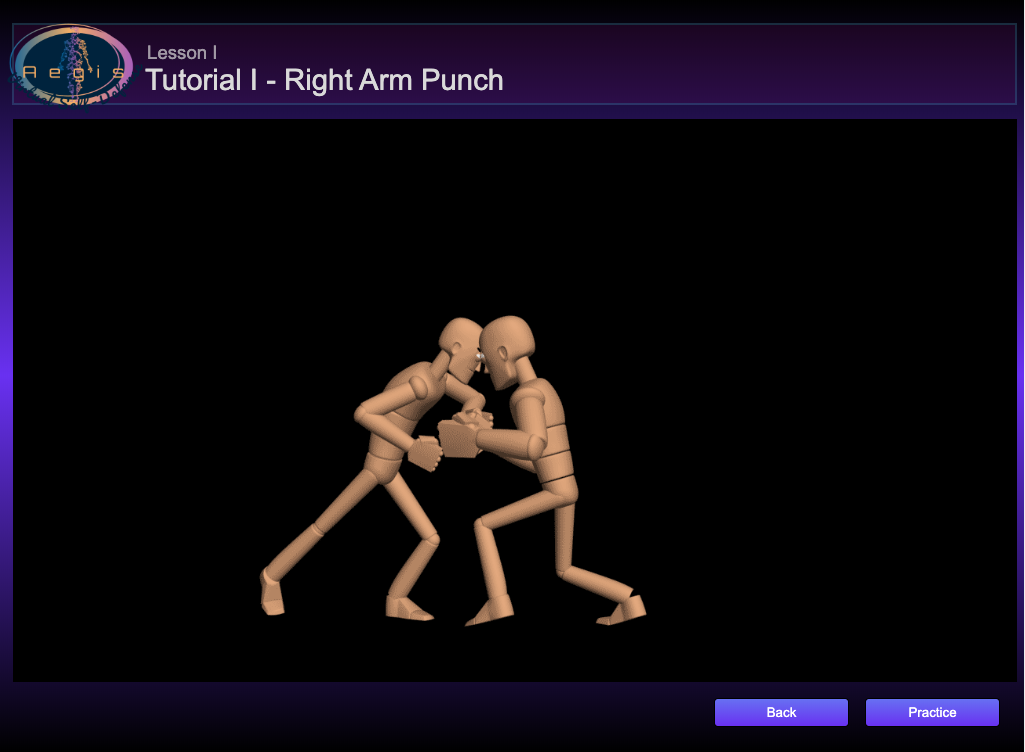
\includegraphics[scale=0.25]{images/Mockups/tutorial.png} \label{fig:tutorial} 
  }
  \caption{Home Screen and Tutorials} 
  \centering
  \label{fig:homeTut}
\end{figure}
\clearpage
Figure \ref{fig:practiceFight} shows screens related to \textit{Practice} and \textit{Fight} sessions. If the user chooses to practice or fight, they will first be asked if they want to do so with a haptic suit as shown in figure \ref{fig:dialogBox}. If the user responds in positive, they will be guided to put their haptic suit on (as shown in figure \ref{fig:haptic}) and will be prompted to calibrate the frequency and amplitude of the haptic signal that they prefer. Figure \ref{fig:practice} and \ref{fig:fight} shows the practice and fight sessions screens. These sessions will start when user clicks the \textit{Start} button. After the session has ended, a feedback report is available on the left.
    \begin{figure}[ht] 
  \subfigure[Haptic Screen]{% 
    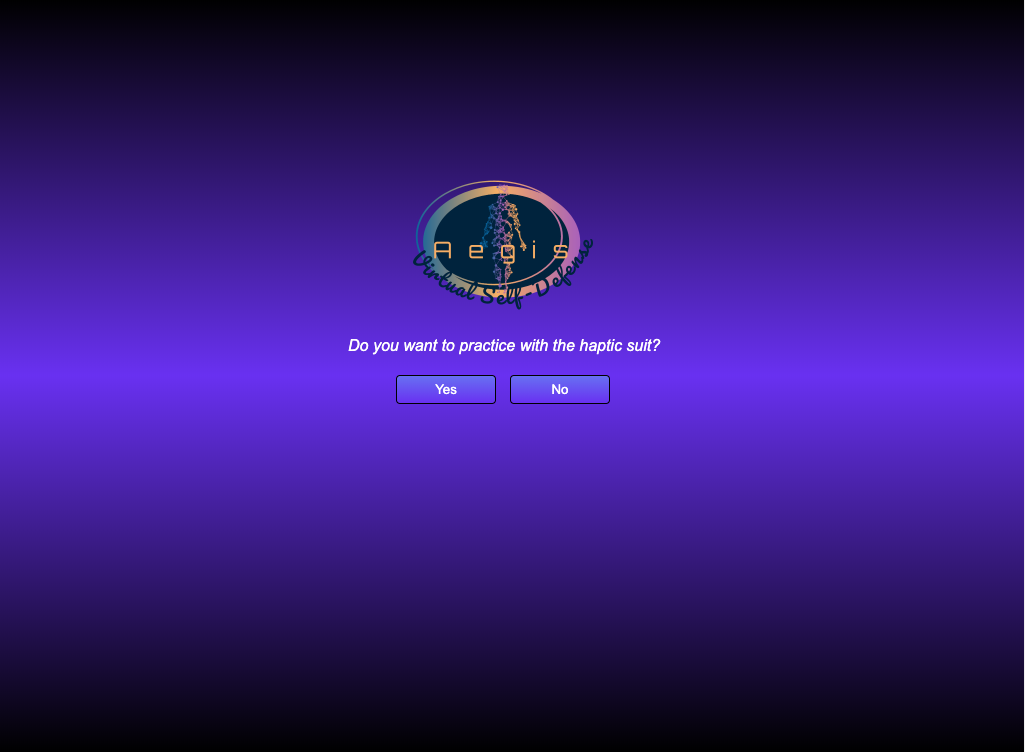
\includegraphics[scale=0.25]{images/Mockups/hapticDialogBox.png} \label{fig:dialogBox} 
  } 
 \quad 
  \subfigure[Haptic Calibration Screen]{% 
    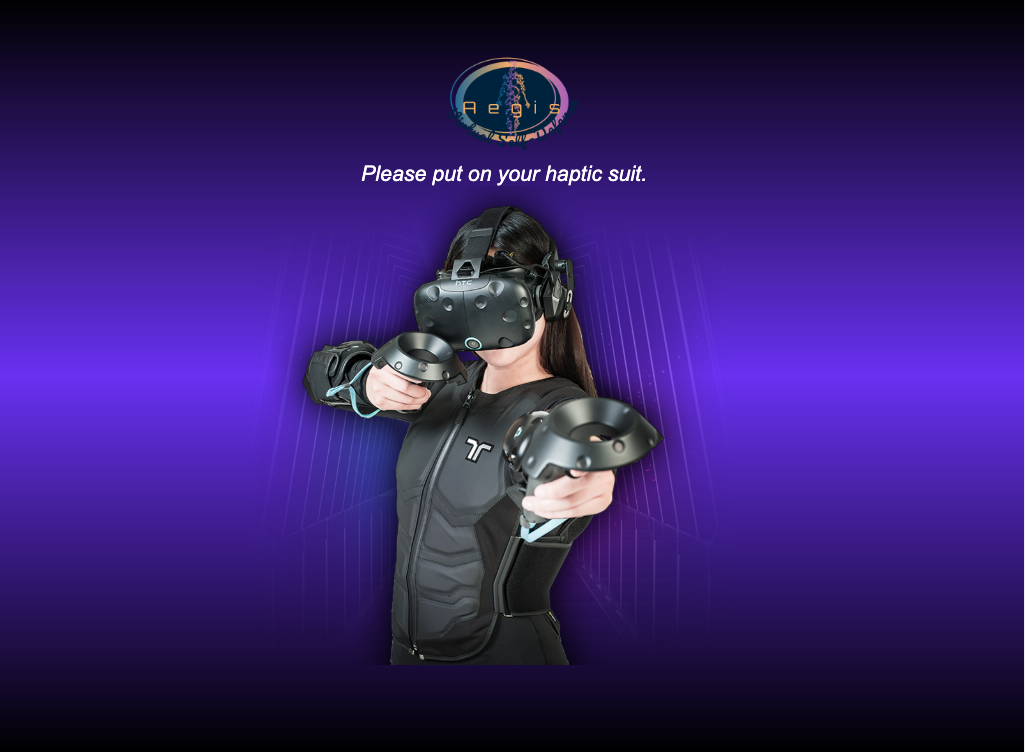
\includegraphics[scale=0.25]{images/Mockups/haptic.png} \label{fig:haptic} 
  } 
  \quad 
  \subfigure[Lesson I Tutorial I: Practice Session Screen]{% 
    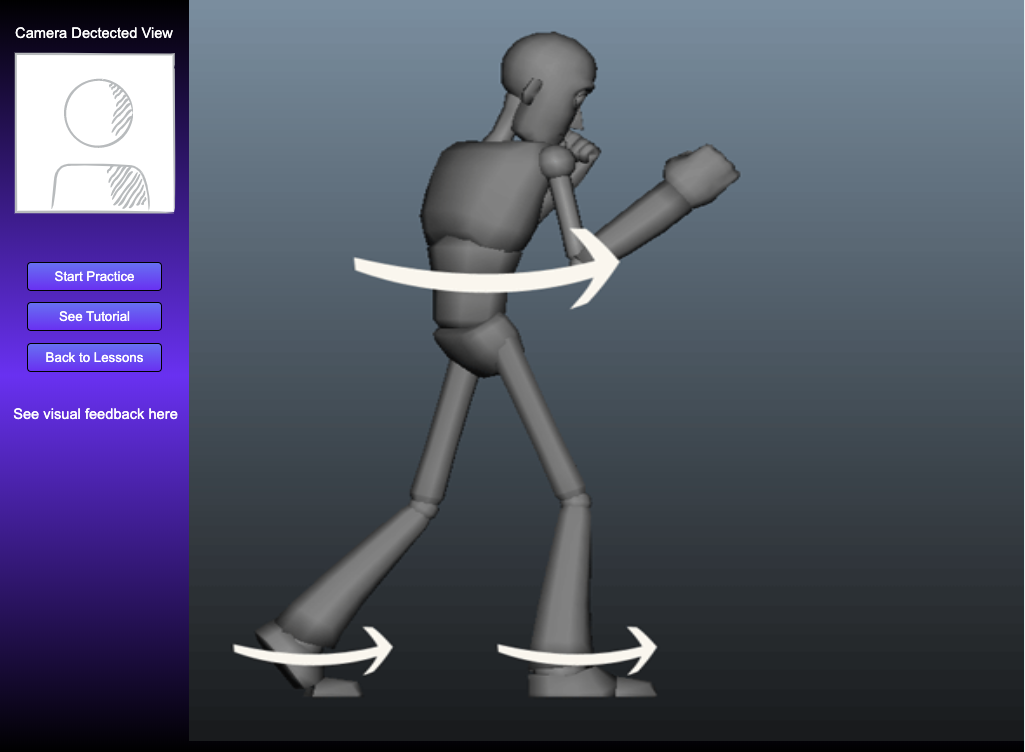
\includegraphics[scale=0.25]{images/Mockups/practice.png} \label{fig:practice} 
  }
  \quad 
  \subfigure[Lesson I: Fight Session Screen]{% 
    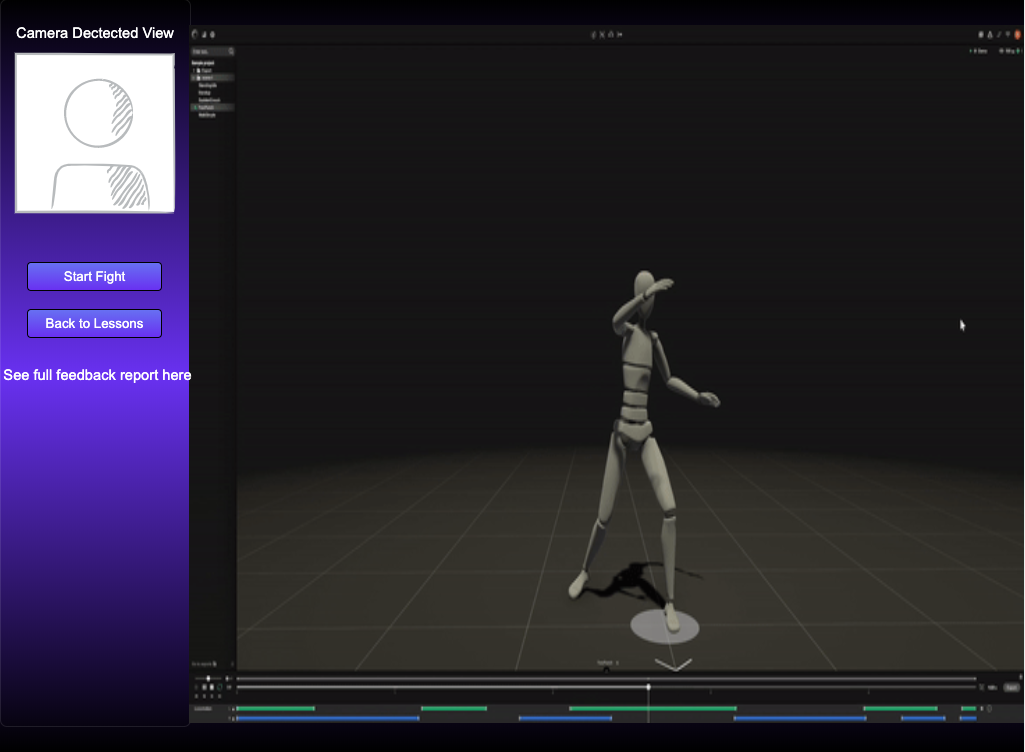
\includegraphics[scale=0.25]{images/Mockups/fight.png} \label{fig:fight} 
  }
  \caption{Practice and Fight Sessions} 
  \centering
  \label{fig:practiceFight}
\end{figure}
\clearpage
\subsection{Application Program Interface (API)}
Not Applicable.
\subsection{Hardware/Communication Interfaces}
Since openpose will capture user's movements through a camera, a built-in camera or webcam is required. 
\\
All the hardware will require a connection with power source (9V battery) to power micro-controller, EMS (Electrical Muscle Stimulator) and tens machine.
\\
The Micro-controller will take decisions based on feature and pose vector to on and off some switches which control the tens machine and EMS.
\\
All the communication between hardware and software will be done serially, hence a serial communication cable will be required to transmit and receive data. 
\section{Use Cases}
Figure \ref{fig:usecase} shows the use case diagram of the project, which comprises of the functionalities of the system with respect to the user perspective. \\ \\ 
Following is a short description of the diagram: \\ \\
User can login/sign-up into the system and will be granted access after verification of credentials. After that they can either choose \textit{Train Mode} or \textit{Fight Mode}. The \textit{Train Mode} further includes animated tutorials and practice sessions. Both fight sessions and practice sessions provide user feedback indicating how well the user performed and how he can improve it. In addition to feedback, fight session also suggest tutorials based on areas the system thinks user has performed poorly. In case a user is fighting or practicing with haptics, they first need to calibrate the frequency and amplitude of the signal at which they are most comfortable. 
\begin{figure}[ht]
    \centering
    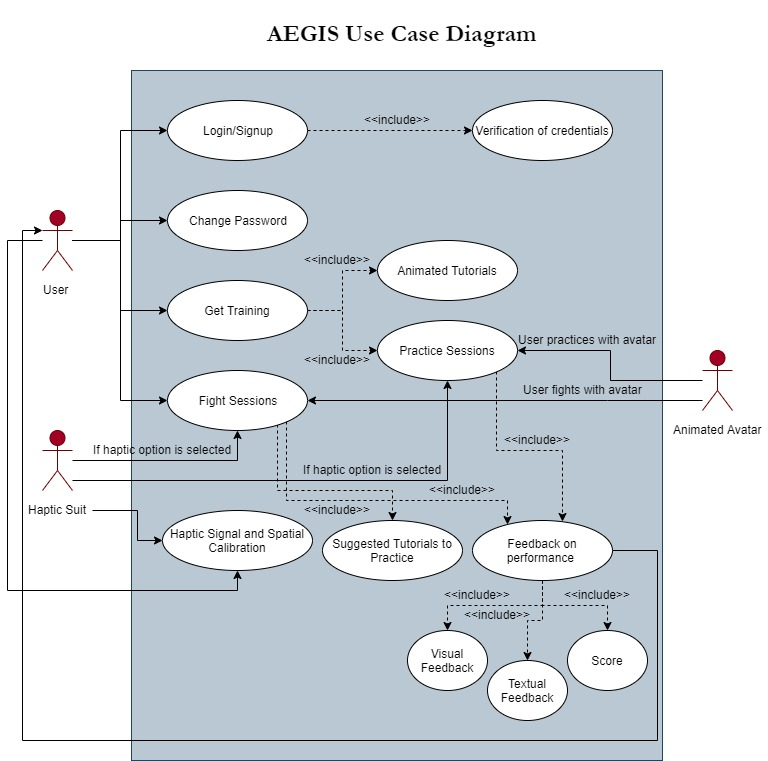
\includegraphics[scale=0.7]{images/UseCaseDiagram.jpg}
    \caption{Use Case Diagram}
    \label{fig:usecase}
\end{figure}
\section{Datasets}
There are no external datasets being used in this project. We will be recording our own videos for performed self-defense techniques which will be used as a benchmark for pose evaluation and in similarity comparison for pose classification.
\section{System Diagram}
\begin{figure}
    \centering
    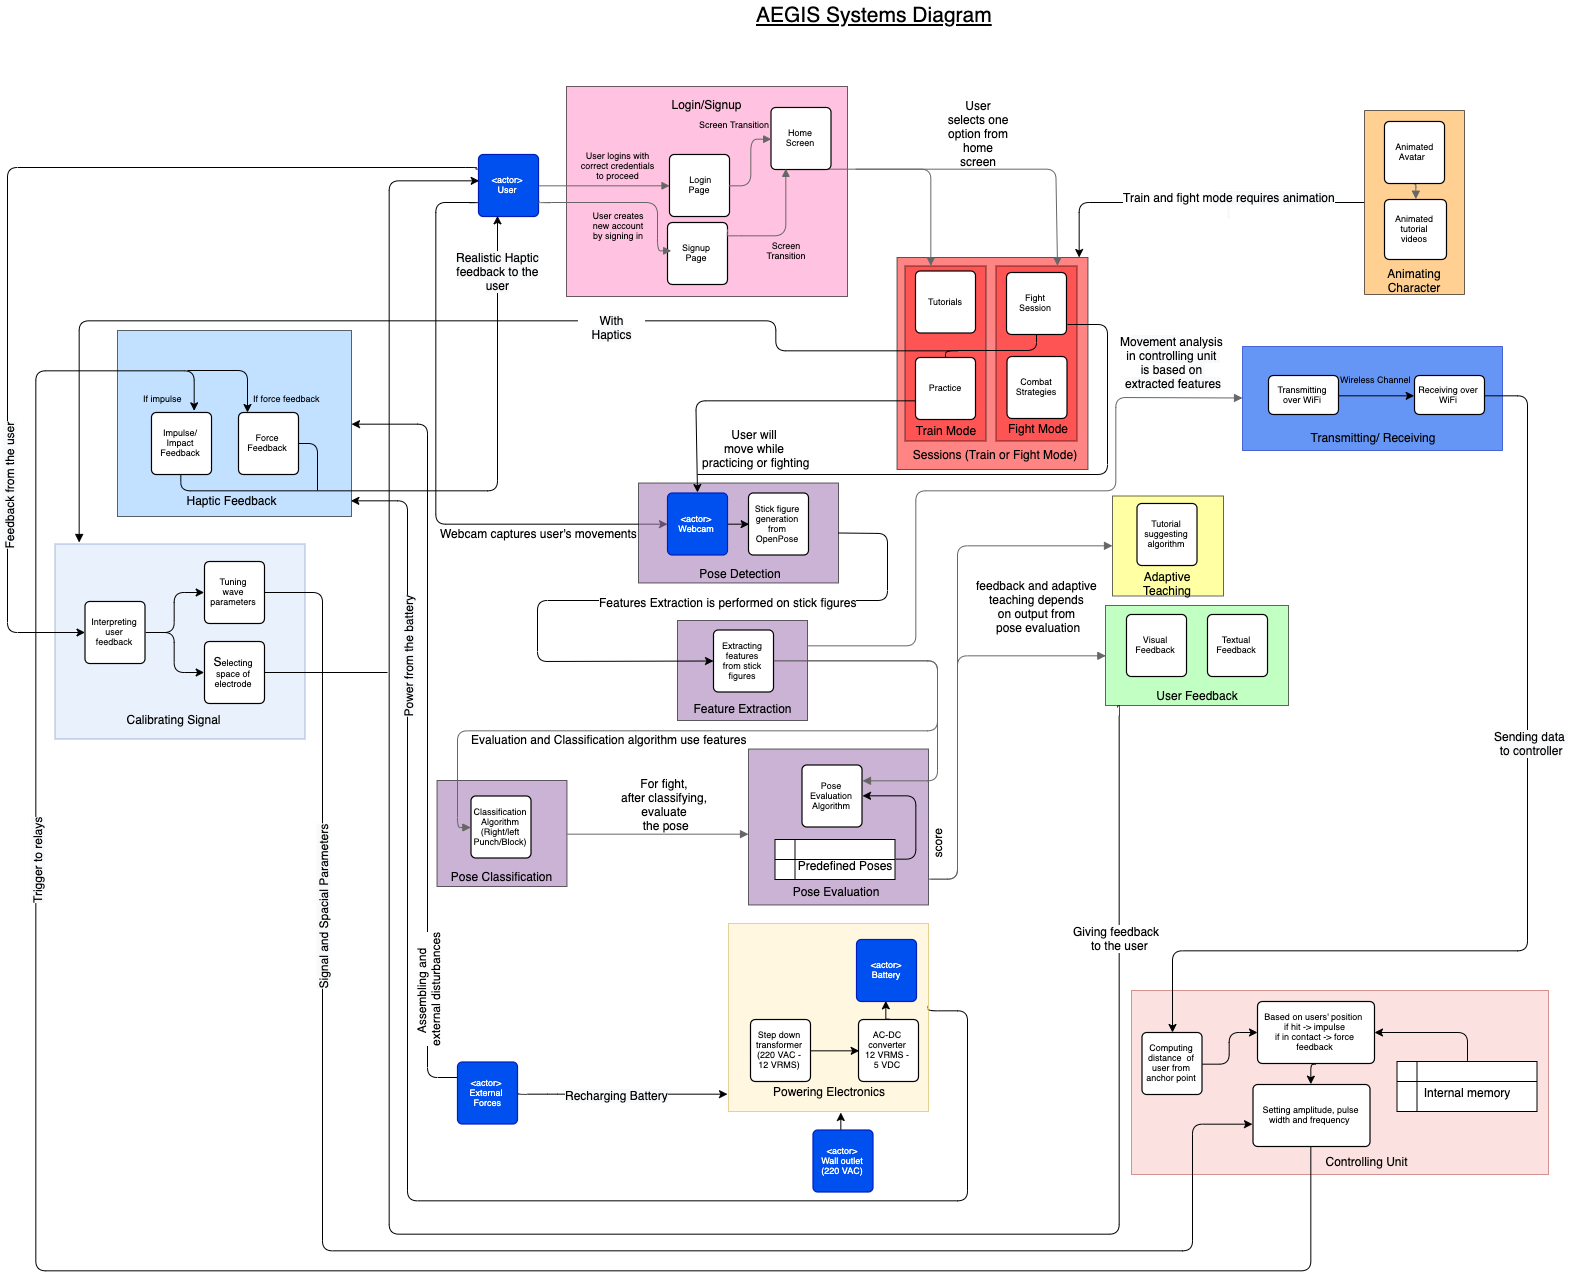
\includegraphics[scale=0.32]{images/SystemDiagram.png}
    \caption{System Diagram}
    \label{fig:systemDiagram}
\end{figure}
\clearpage
Figure \ref{fig:systemDiagram} shows the system diagram of our system which gives a high-level view of the different components of our system and the interactions between them. Each actor, component and the particular tools/technologies/libraries used to build it are described below.
\subsection{User}
User interacts with a few sub-systems in the main system. First of all, the user completes the sign-up or log-in step. This information is stored in the system's database and the process continues to either a \textit{Train Mode} or \textit{Fight Mode}. Hence, user outputs a selected mode, and in addition to that the user also outputs feedback to the calibration protocol if they choose to interact with haptics. The inputs to the user will be the haptic feedback, user feedback and visual display based on which it will interact with the system.
\subsection{Login/SignUp Module}
The input to this module are the user credentials (ID and password), and upon successful login/signup, the user can output a selection between train or fight mode.
\subsection{Animating Character Module}
This block is required to animate the avatar for the tutorials, practice and fight session. This will output the avatar to the tutorials, practice and fight sessions. This block will also animate user's body parts which will be in the view of the camera (like hands). 
\subsection{Sessions Module}
There are two modes that the user will select, either fight or train mode. Train mode is further divided into lessons/animated tutorials and practice sessions, while fight mode contains fight sessions along with avatar's combat strategies. Both the modes require animations from the animation module. 
\subsection{Calibrating Signal Module}
Before these sessions, if the user selects \textit{with haptics} then the haptics component needs to be calibrated. The calibration scheme consists of an automatic protocol that takes in user’s feedback as input to calibrate the parameters of wave (pulse width, frequency and amplitude of the EMS waves). These will be sent to the controlling unit and the controlling unit will tune in the parameters accordingly. Based on this, the output of the haptics will be modified, and the user will rate these modified sensations. This loop will continue until the sensation lies perfectly according to user's comfort. 
\subsection{Controlling Unit Module}
This block is comprised of primarily Arduino or any IoT platform. This will take in inputs over WiFi/cable from the Feature Extraction Module. Based on the feature vector, it will send in triggers and the parameters to the haptic block. This will make decisions as to which haptic signal to activate (impulse or force feedback). Based on distance of the user from the avatar it will activate the relays by comparing the distances with the pre-stored data and conditions in the memory. This also takes part in the calibration scheme where it gets information from the protocol and sets parameters accordingly.
\subsection{Haptic Feedback Module}
This block has two types of outputs, either a force feedback or an impulse feedback. The information about the wave parameters and when to activate comes directly from the Control Unit module. The output is directly exposed to the user. It makes the user feel the virtual environment.
\subsection{Transmission/Receiving Block}
This block gets the output from the feature extraction module and sends the feature vector to the control unit which makes decisions as described in Controlling Unit Module.
\subsection{Pose Detection Module}
This takes images from the webcam as inputs at a certain frequency and outputs a series of time-dependent raw pose vectors in form of JSON files. This will be sent to the feature extraction module.
\subsection{Feature Extraction}
This module takes a series of time-dependent raw pose vectors in form of JSON files as input and outputs features like velocity, rotation. This feature vector/tensor will be sent to the control unit and also to the pose classification block in the case of a fight session, before finally sending it to the pose evaluation module.
\subsection{Pose Evaluation Module}
This block gets input from the feature extraction block. This input feature vector is compared with the benchmark feature vector of predefined pose. Based on this comparison the score is given. The score is then sent to adaptive teaching block and the user feedback block.
\subsection{User Feedback Module}
This block based on the numerical score gives feedback in natural language and also gives visual feedback based on detected stick figures. The feedback will be sent to the display.
\subsection{Adaptive Teaching}
This component suggests the next tutorial based on the current performance score. The input is the score from pose evaluation and the outputs are the suggested tutorials that the user should practice more. 
\subsection{Powering Electronics}
This block recharges the battery and powers the entire circuitry including the haptic suit, the controlling unit, and the desktop (PC). 
\subsection{External Forces}
These are forces used for assembling in order to put the suit together. These are also the disturbances causing noise in webcam images which OpenPose smooths itself. These external forces are at play when the user interacts with it whilst wearing the suit and recharging its battery (plug forces).




